\chapter{Implémentation du protocole}

\section{Solutions choisies}
Le langage choisi est \textsc{JAVA}. Les motivations de ce choix sont les suivantes : la facilité  ainsi que la mise à disposition par \textsc{JAVA} de moniteurs. Effet, la classe \texttt{UnicastRemoteObject} propose les objets \textit{RMI} (Remote Method Invocation). Il s'agit d'objets \og distants \fg{} auxquels des appels de méthodes peuvent être effectués comme si l'objet était local. De plus  l'implémentation des objets \texttt{RMI}  utilise les moniteurs. Ce mécanisme, garantissant l'emploi de canaux de type \texttt{FIFO}, est donc approprié pour le protocole de ce projet.  

\section{Implémentation}

\subsection{Partie serveur}
La partie \og serveur \fg{} est implémentée par la classe \texttt{IA}, la figure \ref{fig:ia} illustre que cette classe hérite de l'interface \texttt{IIA}. Cet héritage est indispensable pour l'utilisation d'objet \texttt{RMI}. Les signatures des méthodes que l'interface contient sont les moyens pour le client de dialoguer avec le serveur. Bien sûr le client doit avoir la connaissance de cette interface.

 \begin{figure}[htb]
   \centering
   
\includegraphics[scale=.5]{img/ia.eps}
   \caption{Partie serveur}
   \label{fig:ia}
 \end{figure}
\clearpage
\paragraph{L'IHM serveur} (\cf{} figure \ref{fig:ihmIA}) est composée de deux parties : 
\begin{enumerate}
\item 
Partie supérieure : Affichage de l'automate serveur.
\item
Partie inférieure : Affichage textuel des événements.
\end{enumerate}
L'utilisateur n'a en théorie aucune interaction possible avec le serveur. Dans un soucis pratique nous avons cependant rajouté un bouton \texttt{QUIT} permettant de quitter et réinitialiser le serveur.
 \begin{figure}[htb]
   \centering
   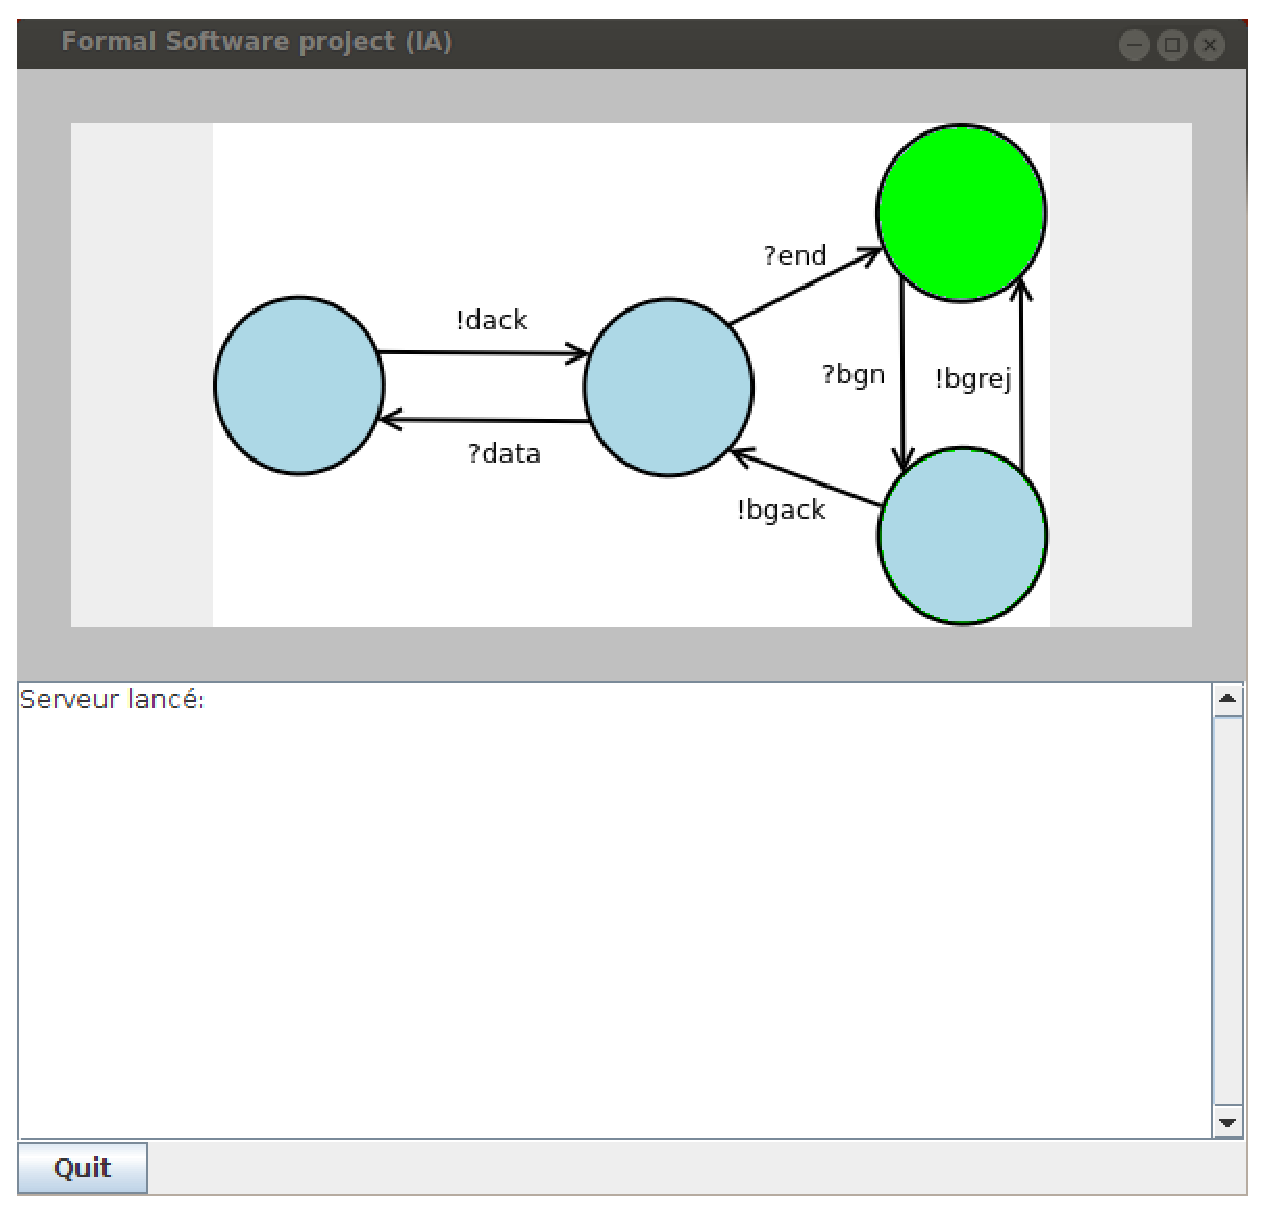
\includegraphics[scale=.5]{img/ihmIA.eps}
   \caption{IHM du serveur}
   \label{fig:ihmIA}
 \end{figure}


\clearpage
\subsection{Partie client}
\paragraph{L'IHM client}(\cf{} figure \ref{fig:ihmCLIENT}) est composée de trois parties : 
\begin{enumerate}
\item 
Partie supérieure : Affichage de l'automate client.
\item
Partie centrale : Affichage textuel des événements.
\item 
Partie inférieure : Boutons de contrôle.
\end{enumerate}

 \begin{figure}[htb]
   \centering
   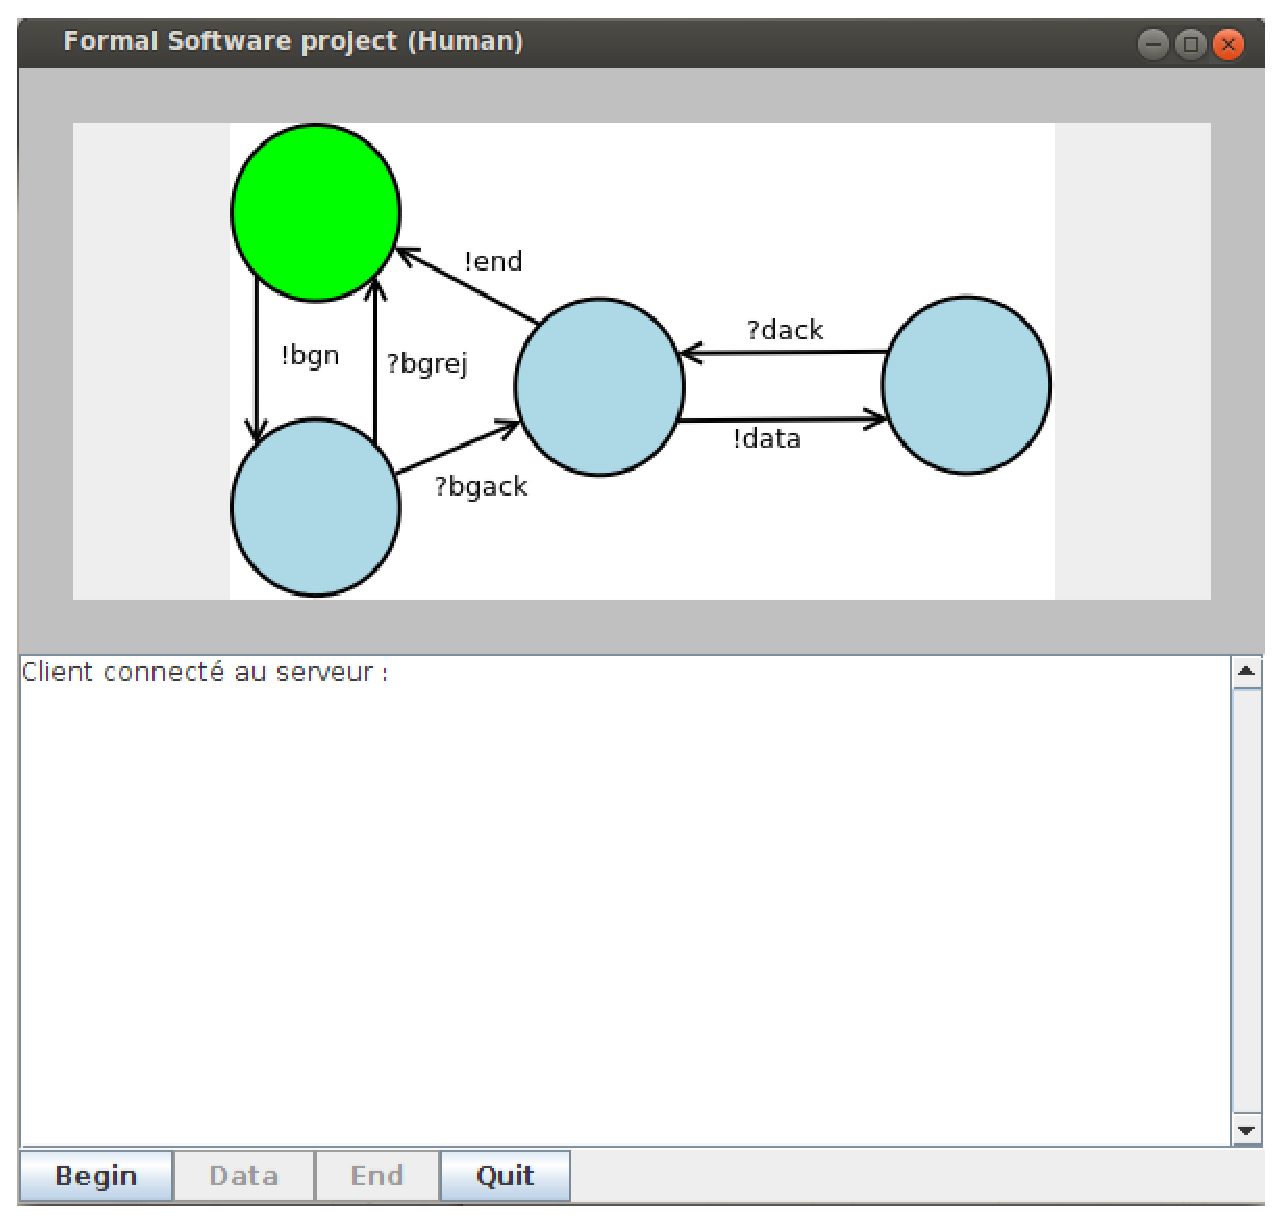
\includegraphics[scale=.5]{img/ihmCLIENT.eps}
   \caption{IHM du client}
   \label{fig:ihmCLIENT}
 \end{figure}
Les boutons de contrôles :  \texttt{BEGIN}, \texttt{DATA} et \texttt{END} correspondent respectivement aux opérations : \texttt{sendBegin()}, \texttt{sendData()} et \texttt{sendEnd()}, définies dans l'interface \texttt{IIA} (\cf{} figure \ref{fig:ia}). L'utilisateur peut par ses boutons \og tirer \fg{} les transitions de l'automate.

\section{Problèmes rencontrés}
\subsection{Mutli-threading}
Au cours du développement de l'application, il était nécessaire d'effectuer systématiquement des tests pour vérifier si les automates étaient dans un état cohérent. Dans un souci pratique nous avons effectué ces tests en local. L'objet \og distant \fg{} \texttt{RMI} était donc lié au \texttt{localhost} (\verb+127.0.0.0+). Ainsi les messages entre le client et le serveur mettaient en moyenne moins d'un millième de seconde pour rejoindre leur destinataire (modulo la précision de l'API de mesure temporelle de \textsc{JAVA}).

\paragraph{}
Un des premiers problèmes que nous avons rencontré dans le développement l'application était donc celui de \og ralentir \fg{} ces opérations afin de vérifier la cohérence des automates.

\paragraph{}
De plus les rafraîchissements des espaces de visualisation des différents automates posèrent eux aussi de nombreux problèmes. La couche \texttt{SWING} de \textsc{JAVA} en charge de l'implémentation des interfaces graphiques, est elle-même un thread à part entière. Une des difficultés était donc de synchroniser au sein d'un même thread application, le thread \og vue \fg{} (la couche \texttt{SWING}) avec la couche \og métier \fg{} (algorithmes des automates et de leurs communications).


% LocalWords:  Implémentation UnicastRemoteObject RMI Remote Method
% LocalWords:  l'implémentation FIFO IA IIA L'IHM QUIT IHM BEGIN END
% LocalWords:  sendBegin sendData sendEnd Mutli-threading localhost
% LocalWords:  modulo l'API thread tread
